%% Chapter 9 : Generation Forecasting using WRF

\section{Introduction to NWP}
\
\
\
\
NWP stands for Numerical Weather Prediction. It uses mathematical models of the atmospheric and oceanic physical processes to predict the weather based on current weather conditions. These numerical solutions are possible due to the the advent of computer simulations. Therefore, though first NWP simulations were attempted in the 1920's realistic results were produced in the 1950's when computer simulation technology improved.\\

Many different global (predicting weather for entire earth) and regional (predicting weather for a particular region) forecast models are run in different countries worldwide. The current weather data for the initialization of these NWP models are acquired from radiosondes, weather satellites and other observing systems.\\

The NWP models use systems of differential equations based on the laws of physics, fluid motion, and chemistry, and use a coordinate system which divides the planet into a 3D grid. Winds, heat transfer, solar radiation, relative humidity, and surface hydrology are calculated within each grid cell, and the interactions with neighboring cells are used to calculate atmospheric properties in the future. These models can be used for both short-term forecasting for predicting weather as well as long-term forecasts for understanding the trend of climate change.\\

The mathematical models themselves are are chaotic due to the presence of partial differential equations that govern the atmospheric and oceanic physical processes. To solve these complex and chaotic equations with the vast datasets (initializing dynamic weather data and static geographical data)NWP's require sumpercomputer architectures for computing solutions. On the contrary, it is impossible to solve these equations exactly even with huge supercomputers, and the errors in the simulation grow with time. Moreover, parameterizations (replacing processes that are too small-scale or complex to be physically represented in the model by a simplified process) for various physical processes is also required for faster and more accurate simulations. Hence, with the present understanding of the NWP's, we can assume that accurate forecasts are generated to about 14 days even with perfectly accurate initializing data and a perfect model.\\

\section{The WRF NWP Model} 
\
\
\
\
The WRF or the Weather Research and Forecasting is a NWP system developed by a conglomerate of atmospheric and oceanic research institutions. The principal institutions are: National Center for Atmospheric Research (NCAR), the National Oceanic and Atmospheric Administration (represented by the National Centers for Environmental Prediction (NCEP) and the (then) Forecast Systems Laboratory (FSL)), the Air Force Weather Agency (AFWA), the Naval Research Laboratory (NRL), the University of Oklahoma (OU), and the Federal Aviation Administration (FAA). The bulk of the work on the model has been performed or supported by NCAR, NOAA, and AFWA.\\

The WRF has two dynamical (computational) cores (or solvers; ARW [Advanced Research WRF] developed by NCAR and the WRF-NMM [Nonhydostatic Mesoscale Model] developed by NCEP), a data assimilation system, and a software architecture allowing for parallel computation and system extensibility. The model serves a wide range of meteorological applications across scales ranging from meters to thousands of kilometers.

Being an open-source and community driven software, it has been adopted by many forecasting centers internationally. Moreover, there are about 23,000 registered WRF users in over 150 countries making the community strong and vibrant; which extends to the forums making them rich n content and hence easy to debug WRF simulation problems.\\


\section{WRF Software Components}
\
\
\
\
The Fig (\ref{figc10h1}) shows the software architecture of the WRF-ARW system.

\begin{figure}[H]
\centering
\includegraphics[scale=0.30]{WRF_1}
\caption{WRF-ARW Software Architecture}
\label{figc10h1} %% to refer use, \ref{}
\end{figure}

The brief overview of the major WRF system programs is as follows;\\

\begin{enumerate}

\item \blindtext 	\textbf{WPS:} This program is used primarily for real-data simulations. Its functions include 1) defining
simulation domains; 2) interpolating terrestrial data (such as terrain, landuse, and soil types) to the simulation domain; and 3) degribbing and interpolating meteorological data
from another model to this simulation domain.

\item \blindtext \textbf{WRF-DA:} This program is optional, but can be used to ingest observations into the interpolated
analyses created by WPS. It can also be used to update WRF model's initial conditions
when the WRF model is run in cycling mode.

\item \blindtext \textbf{ARW Solver:} This is the key component of the modeling system, which is composed of several
initialization programs for idealized, and real-data simulations, and the numerical
integration program.

\item \blindtext \textbf{Post-Processing & Visualization Tools:} Several programs are supported, including RIP4 (based on NCAR Graphics), NCAR
Graphics Command Language (NCL), and conversion programs for other readily
available graphics packages like GrADS. Program VAPOR, Visualization and Analysis Platform for Ocean, Atmosphere, and
Solar Researchers, is a 3-dimensional data visualization
tool, and it is developed and supported by the VAPOR team at NCAR.Program MET, Model Evaluation Tools , is
developed and supported by the Developmental Test bed Center at NCAR.

\end{enumerate}

We will not be using the WRF-DA and the Post-Processing & Visualization Tools  software as we will not be doing data assimilation, and e have developed a visualization and data extraction application in MATLAB to suit our needs. We will be using the WPS and the WRF-ARW Solver for performing day-ahead short-term weather forecasting for a real data case. \\

The detailed overview of the component programs of the WPS and the WR-ARW solver along with the step-wise implementation will be discussed in the subsequent sections of the text.\\

\newpage

\section{Real Data Case Short-Term Weather Forecasting using WPS and WRF-ARW Solver}
\
\
\
\
The Fig (\ref{figc10h2}) illustrates the step-wise implementation of the WPS and WRf programs for simulating a real data case.

\begin{figure}[H]
\centering
\includegraphics[scale=0.9]{WRF_22}
\caption{WPS and WRF Step-Wise Implementation Scheme}
\label{figc10h2} %% to refer use, \ref{}
\end{figure}

\subsection{WPS Program Components}
\
\
\
\
The WRF Preprocessing System (WPS) is a set of three programs whose collective role is
to prepare input to the real program for real-data simulations. Each of the programs
performs one stage of the preparation: geogrid defines model domains and interpolates
static geographical data to the grids; ungrib extracts meteorological fields from GRIBformatted
files; and metgrid horizontally interpolates the meteorological fields extracted
by ungrib to the model grids defined by geogrid. The work of vertically interpolating
meteorological fields to WRF eta levels is performed within the real program.\\

\begin{enumerate}

\item \blindtext \textbf{Program Geogrid:} The purpose of geogrid is to define the simulation domains, and interpolate various
terrestrial data sets to the model grids. The simulation domains are defined using
WPS
WRF-ARW V3: User’s Guide 3-3
information specified by the user in the “geogrid” namelist record of the WPS namelist
file, namelist.wps. 	

\item \blindtext \textbf{Program Ungrib:} The ungrib program reads GRIB files, "degribs" the data, and writes the data in a simple
format called the intermediate format. The GRIB files contain time-varying meteorological
fields and are typically from another regional or global model, such as NCEP's NAM or
GFS models. The ungrib program can read GRIB Edition 1 and, if compiled with a
"GRIB2" option, GRIB Edition 2 files. 

\item \blindtext \textbf{Program Metgrid:} The metgrid program horizontally interpolates the intermediate-format meteorological
data that are extracted by the ungrib program onto the simulation domains defined by the
geogrid program. The interpolated metgrid output can then be ingested by the WRF real
program.

\end{enumerate}

\subsection{WRF Program Components}
\
\
\
\
The WRF model is a fully compressible and nonhydrostatic model (with a run-time
hydrostatic option). Its vertical coordinate is a terrain-following hydrostatic pressure
coordinate. The grid staggering is the Arakawa C-grid. The model uses the Runge-Kutta
2nd and 3rd order time integration schemes, and 2nd to 6th order advection schemes in
both the horizontal and vertical. It uses a time-split small step for acoustic and gravitywave
modes. The dynamics conserves scalar variables.

\begin{enumerate}

\item \blindtext \textbf{real.exe:} It converts the output files from metgrid program of the WPS system into a format which can be used as an initialization for the wrf.exe	

\item \blindtext \textbf{wrf.exe:} It is the numerical integration program which solves the partial differential equations of the atmospheric and oceanic processes to compute the weather forecasts.	

\end{enumerate}

\newpage

\section{Computing Platform to Run WRF}
\
\
\
\
For running the the WRF software a 4-Node Raspberry-Pi2 (RPi) cluster has been developed, to provide for the distributed computation environment which makes the WRF simulations faster.
  
\subsection{Raspberry-Pi2 Micro-Computer}
\
\
\
\
It is a single-board micro-computer developed by the Raspberry Pi Foundation in the United Kingdom. Its primary purpose is to serve as a low priced tool for teaching and learning computer science. However, due its inexpensiveness and the broad spectrum of capabilities has made it a favourite of hobbyists, computer enthusiasts, students and researchers for embedded development. As it has an ARMv7 processor, it can run a full range of ARM GNU/Linux distributions.\\

\textbf{Hardware}:

\begin{itemize}

\item A 900MHz Quad-Core ARM Cortex-A7 CPU

\item 1GB RAM

\item 4 USB Ports

\item 40 GPIO (General Purpose Input/Output) pins

\item Full HDMI Port

\item Ethernet Port

\item Combined 3.5mm Audio Jack and Composite Video

\item Camera Interface (CSI)

\item Display Interface (DSI)

\item Micro SD Card slot

\item VideoCore IV Graphics Core	

\end{itemize}

\textbf{Software (Operating Systems):}:

\begin{itemize}

\item RASPBIAN

\item UBUNTU MATE

\item SNAPPY UBUNTU CORE

\item WINDOWS 10 IOT CORE

\item OSMC

\item OPENLECPINETRISC OS

\end{itemize}

\subsection{Setting up Raspberry Pi Cluster for WRF}
\
\
\
\
The Fig (\ref{figc10h3}) gives the step-wise instructions to develop a cluster of Raspberry-Pi2 micro-computers to run the WRF software

\begin{figure}[H]
\centering
\includegraphics[scale=1]{WRF_33}
\caption{Flow Diaram for Setting up Raspberry Pi Cluster for WRFe}
\label{figc10h3} %% to refer use, \ref{}
\end{figure}

\textbf{Set up a Single RPi:
}

\begin{enumerate} 

\item \blindtext Components required are: 1 × Raspberry Pi, 1 × 32GB Micro SD Card, 1 × Card Reader, 1 × USB Power Cable, 1 × USB Power Hub, 1 × HDMI Cable, 1 × USB Mouse, 1 × USB Keyboard and  1 × HDMI compatible Display.

\item \blindtext Download the RASPBIAN-OS from the Raspberry Pi website (free).

\item \blindtext Download SD Formatter Software from internet (free).

\item \blindtext Download Win32DiskImager Software from the internet (free).

\item \blindtext Format the 32GB Micro SD Card using SD Formatter software.

\item \blindtext Write the downloaded RASPBIAN-OS image to the 32GB Micro SD Card using the Win32DiskImager software.

\item \blindtext Insert the SD card in the RPi.

\item \blindtext Connect the USB Power Hub to the Power source, and the USB Power Cable to the USB Power Hub.

\item \blindtext Attach the USB mouse and keyboard to the USB ports of the RPi.

\item \blindtext Connect the HDMI cable from the RPi to the display screen.

\item \blindtext Power up the RPi by connecting the USB Power Cable to the Micro USB Power port of the Rpi.

\item \blindtext The Rpi will boot; Username – pi and Password – raspberry.

\item \blindtext Go to the configuration menu and do the following:

\begin{enumerate} 

	\item \blindtext Change the Hostname to Pi01

	\item \blindtext Enable SSH

	\item \blindtext Expand storage system
	
	\item \blindtext You may or may not overclock the RPi
	
\end{enumerate}	

\item \blindtext Reboot the Pi

\item \blindtext Shutdown the Rpi.


\end{enumerate}

\textbf{Remote Access RPi:
}\\

Remote access means, able to control RPi without additional display, mouse and keyboard. We will control the RPi via our workstation (Laptop/Desktop) using SSH (Secure Shell).

\begin{enumerate}

\item \blindtext 

\item \blindtext Components required are: LAN Cable
Download Putty software from the internet (free).

\item \blindtext Find out the IP address of the Ethernet port of the workstation and note it down.

\item \blindtext Take out the SD Card from the RPi, using the SD Card Reader to read into its boot partition and add xxx.xxx.xxx.RPi::xxx.xxx.xxx.PC at the end of the cmdline.txt file. Where the first part is the IP static address of the RPi which is set to be in the network space of the workstation’s IP address, and the second part after the double colons is the IP address of the workstation which was found out earlier.

\item \blindtext Now put the SD Card back into the RPi connect it to the workstation via a LAN cable and power it up.

\item \blindtext Open Putty software.

\item \blindtext In the Hostname field enter the Static IP address of our RPi, in the Port field enter 22, and give a name to this configuration and save with the hostname of our RPi i.e. Pi01.

\item \blindtext Now select the hostname of the RPi from the list, press Load and the press open.

\item \blindtext A terminal window will open, giving us a terminal access to our RPi.


\end{enumerate}

\textbf{Share Internet with RPi 
}

\begin{enumerate}

\item \blindtext From now on we will be using the RPi through SSH.

\item \blindtext We will share the internet (WiFi) of workstation with the RPi through the Ethernet port where it is connected.

\item \blindtext In a Windows system, this can be done by going to the \textit{Networks and Sharing} Option of the Control Panel.

\item \blindtext Go to the Change Adapter Settings page.

\item \blindtext There Right-Click on the WiFi icon which shows internet connectivity and hit Properties.

\item \blindtext Navigate to the \textit{Sharing} Tab and select the\textit{ Allow other users to connect through this computer’s Internet connection} checkbox.

\item \blindtext Now Right-Click on the \textit{LAN Adapter} and hit \textit{Properties}. Double click the \textit{IPV4} option and verify that some dynamic IP is populated. The IP address of the RPi should be within this IP addresses range.

\item \blindtext After this you can power up the RPi and connect to the workstation via the LAN cable.

\item \blindtext Now using Putty’s terminal we can have internet access in the RPi which is shared from the workstation. (Check connectivity using ping www.google.com)


\end{enumerate}

\textbf{Build WRF Software on RPi
}

\begin{enumerate}

\item \blindtext Download the TAR file of the WRF (Weather Research and Forecasting) and WPS (WRF Pre-processing System) from the WRF model site. Also download static geographic data used along with WPS and WRF from the UCAR EDU website.

\item \blindtext Download Filezilla Software from the internet (free).
 
\item \blindtext Run the RPi through SSH on the workstation, transfer the downloaded TAR files from the workstation to the RPi using the Filezilla software.

\item \blindtext Use the WRF Build Scripts developed to build and install WRF system on the RPi.

\item \blindtext Power off the RPi and remove the SD Card.

\item \blindtext Using the SD Card Reader and the Win32DiskImager; create an image of the SD Card, and store it in the workstation

\end{enumerate}

\textbf{Set up RPi Cluster
}

\begin{enumerate}



\item \blindtext Components required are: 4 × Raspberry Pi, 4 × 32GB Micro SD Cards, 1 × Card Reader, 4 × USB Power Cables, 4 × LAN Cables, 2 × USB Power Hub, 1 × Extension Box.

\item \blindtext Using the SD Card reader and the Win32DiskImager software, burn the image which was earlier stored on the workstation (with installed WRF) onto to the rest of the SD Cards.

\item \blindtext Now, for each of the new SD Cards using the SD Card Reader read into its boot partition and add xxx.xxx.xxx.RPi::xxx.xxx.xxx.PC at the end of the cmdline.txt file. Where the first part is the IP static address of the RPi which is set to be in the network space of the workstation’s IP address, and the second part after the double colons is the IP address of the workstation which was found out earlier. Make sure that all the IP addresses are unique.

\item \blindtext Put the SD Cards in the respective RPi’s.

\item \blindtext Connect all the RPi’s and the workstation to the Network Switch via LAN Cables.

\item \blindtext Connect all the RPi’s to the Power USB Hubs using the USB Power Cables.

\item \blindtext Connect the workstation, the Network Switch and the Power USB Hubs to the Power Source, switch on the Power Source.

\item \blindtext Using Putty softare to SSH into all the RPi’s create a passwordless SSH between them.

\item \blindtext Create a machine file in each of the RPi’s home directory.

\item \blindtext The RPi cluster is ready to use.

\end{enumerate}

The Fig (\ref{figc10h4}) illustrates the schematic of the 4-Node Raspberry-Pi2 Cluster developed for running the WRF software in a cluster environment so as to use its parallel computation feature  to its full potential.

\begin{figure}[H]
\centering
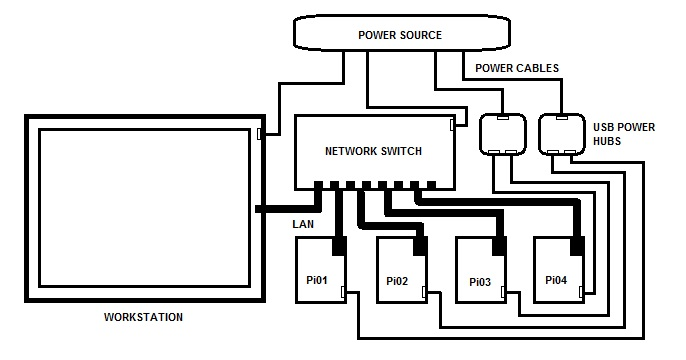
\includegraphics[scale=1]{RPiCluster_IMG1}
\caption{Schematic: 4-Node Raspberry-Pi2 Cluster }
\label{figc10h4} %% to refer use, \ref{}
\end{figure}

The results of energy forecasting using WRF software are presented in the next section.In addition, a GUI based application for visualization and extraction of forecasted weather variables from the WRF NETCDF output files is developed in MATLAB, the application GUI can be found in the Appendix. 

\newpage

\section{Results}

\subsection{4-Node Raspberry-Pi2 Cluster for Running WRF}
\
\
\
\
The Fig (\ref{}) shows the working 4-Node Raspberry-Pi2 Cluster on my desk in GERMI.

\begin{figure}[H]
\centering
\includegraphics[scale=0.20]{WRFCluster1}
\caption{Schematic: 4-Node Raspberry-Pi2 Cluster }
\label{figc10h4} %% to refer use, \ref{}
\end{figure}



\subsection{WRF Namelist Files}
\
\
\
\
\
Name-List files provide for options used to customize the WRF simulation, it is through changing the parameters in these files that the WRF can be run as desired by the user. The WRF software has two name-list files: namelist.wps and namelist.output which are given in the Tables (\ref{WRFTab1},\ref{WRFTab2}).\\

The namelist.wps file is used by the WPS software. It providing options for customizing the geogrid.exe, ungrib.exe and metgrid.exe application components.\\

The namelist.output file is used by the WRF software. It provides options for customizing the model run duration, numerical integration parameters, physics options and nesting parameters.


\newpage

\begin{table}[H]
  \centering
  \caption{namelist.wps Options Table}
    \begin{tabular}{|l|l|}
    \hline
    \multicolumn{2}{|c|}{\textbf{namelist.wps-GSEC 1MW}} \bigstrut\\
    \hline
    \multicolumn{1}{|c|}{\textbf{Namelist Variables}} & \multicolumn{1}{c|}{\textbf{Values}} \bigstrut\\
    \hline
    \textbf{\&share} &  \bigstrut\\
    \hline
    wrf\_core & ARW', \bigstrut\\
    \hline
    max\_dom  & 2, \bigstrut\\
    \hline
    interval\_seconds  & 21600 \bigstrut\\
    \hline
    \textbf{\&geogrid} &  \bigstrut\\
    \hline
    parent\_id & 1,   1, \bigstrut\\
    \hline
    parent\_grid\_ratio & 1,   3, \bigstrut\\
    \hline
    i\_parent\_start & 1,   2, \bigstrut\\
    \hline
    j\_parent\_start & 1,   2, \bigstrut\\
    \hline
    s\_we               & 1,   1, \bigstrut\\
    \hline
    e\_we               & 13,  28, \bigstrut\\
    \hline
    s\_sn               & 1,   1, \bigstrut\\
    \hline
    e\_sn               & 13,  28, \bigstrut\\
    \hline
    geog\_data_res      & 10m','10m', \bigstrut\\
    \hline
    dx & 3000, \bigstrut\\
    \hline
    dy  & 3000, \bigstrut\\
    \hline
    map\_proj  & 'lambert', \bigstrut\\
    \hline
    ref\_lat  &  23.275, \bigstrut\\
    \hline
    ref\_lon  & 72.682, \bigstrut\\
    \hline
    truelat1 &  30.0, \bigstrut\\
    \hline
    truelat2 & 60.0, \bigstrut\\
    \hline
    stand\_lon & -98.0, \bigstrut\\
    \hline
    geog\_data\_path  & '/mnt/USB/WPS_GEOG/' \bigstrut\\
    \hline
    \textbf{\&ungrib} &  \bigstrut\\
    \hline
    out\_format  & 'WPS', \bigstrut\\
    \hline
    prefix  & 'FILE', \bigstrut\\
    \hline
    \textbf{\&metgrid} &  \bigstrut\\
    \hline
    fg\_name & 'FILE' \bigstrut\\
    \hline
    io\_form\_metgrid & 2, \bigstrut\\
    \hline
    \end{tabular}%
  \label{WRFTab1}%
\end{table}%

\newpage

\begin{table}[H]
  \centering
  \caption{namelist.output Options Table}
    \begin{tabular}{|l|l|}
    \hline
    \multicolumn{2}{|c|}{\textbf{namelist.output-GSEC 1MW}} \bigstrut\\
    \hline
    \multicolumn{1}{|c|}{\textbf{Namelist Variables}} & \multicolumn{1}{c|}{\textbf{Values}} \bigstrut\\
    \hline
    \textbf{\&time\_control} &  \bigstrut\\
    \hline
    run\_days & 0, \bigstrut\\
    \hline
    run\_hours                            & 24, \bigstrut\\
    \hline
    run\_minutes                          & 0, \bigstrut\\
    \hline
    run\_seconds                          & 0, \bigstrut\\
    \hline
    end\_hour                             & 00,   00,   12, \bigstrut\\
    \hline
    end\_minute                           & 00,   00,   00, \bigstrut\\
    \hline
    end\_second                           & 00,   00,   00, \bigstrut\\
    \hline
    interval\_seconds                     & 21600 \bigstrut\\
    \hline
    input\_from\_file                      & .true.,.true.,.true., \bigstrut\\
    \hline
    history\_interval                     & 15,  15,   60 \bigstrut\\
    \hline
    frames\_per\_outfile                   & 1000, 1000, 1000, \bigstrut\\
    \hline
    restart  & .false., \bigstrut\\
    \hline
    restart\_interval & 5000, \bigstrut\\
    \hline
    io\_form\_history                      & 2 \bigstrut\\
    \hline
    io\_form\_restart                      & 2 \bigstrut\\
    \hline
    io\_form\_input                        & 2 \bigstrut\\
    \hline
    io\_form\_boundary                     & 2 \bigstrut\\
    \hline
    debug\_level                          & 0 \bigstrut\\
    \hline
    \textbf{\&domains} &  \bigstrut\\
    \hline
    time\_step        & 18,       \bigstrut\\
    \hline
    time\_step\_fract\_num                  & 0, \bigstrut\\
    \hline
    time\_step\_fract\_den                  & 1, \bigstrut\\
    \hline
    max\_dom                              & 2, \bigstrut\\
    \hline
    e\_we                                 & 13,    28,   94, \bigstrut\\
    \hline
    e\_sn                                 & 13,    28,    91, \bigstrut\\
    \hline
    e\_vert                               & 28,    28,    28, \bigstrut\\
    \hline
    p\_top\_requested                      & 5000, \bigstrut\\
    \hline
    num\_metgrid\_levels                   & 32, \bigstrut\\
    \hline
    \end{tabular}%
  \label{WRFTab2}%
\end{table}%

\newpage

\begin{table}[H]
  \centering
  
    \begin{tabular}{|l|l|}
    \hline
    \multicolumn{2}{|c|}{\textbf{namelist.output-GSEC 1MW}} \bigstrut\\
    \hline
    \multicolumn{1}{|c|}{\textbf{Namelist Variables}} & \multicolumn{1}{c|}{\textbf{Values}} \bigstrut\\
    \hline
    num\_metgrid\_soil\_levels              & 4, \bigstrut\\
    \hline
    dx  & 3000, 1000,  3333.33, \bigstrut\\
    \hline
    dy  & 3000, 1000,  3333.33, \bigstrut\\
    \hline
    grid\_id                              & 1,     2,     3, \bigstrut\\
    \hline
    parent\_id                            & 0,     1,     2, \bigstrut\\
    \hline
    i\_parent\_start                       & 1,     2,    30, \bigstrut\\
    \hline
    j\_parent\_start                       & 1,     2,    30, \bigstrut\\
    \hline
    parent\_grid\_ratio                    & 1,     3,     3, \bigstrut\\
    \hline
    parent\_time\_step\_ratio               & 1,     3,     3, \bigstrut\\
    \hline
    feedback  & 1, \bigstrut\\
    \hline
    smooth\_option                        & 0 \bigstrut\\
    \hline
    \textbf{\&physics} &  \bigstrut\\
    \hline
    mp\_physics                           & 3,     3,     3, \bigstrut\\
    \hline
    ra\_lw\_physics                        & 1,     1,     1, \bigstrut\\
    \hline
    ra\_sw\_physics                        & 1,     1,     1, \bigstrut\\
    \hline
    radt                                 & 30,    30,    30, \bigstrut\\
    \hline
    sf\_sfclay\_physics                    & 1,     1,     1, \bigstrut\\
    \hline
    sf\_surface\_physics                   & 2,     2,     2, \bigstrut\\
    \hline
    bl\_pbl\_physics                       & 1,     1,     1, \bigstrut\\
    \hline
    bldt & 0,     0,     0, \bigstrut\\
    \hline
    cu\_physics                           & 1,     1,     0, \bigstrut\\
    \hline
    cudt                                 & 5,     5,     5, \bigstrut\\
    \hline
    isfflx                               & 1, \bigstrut\\
    \hline
    ifsnow                               & 0, \bigstrut\\
    \hline
    icloud                               & 1, \bigstrut\\
    \hline
    surface\_input\_source                 & 1, \bigstrut\\
    \hline
    num\_soil\_layers                      & 4, \bigstrut\\
    \hline
    sf\_urban\_physics                     & 0,     0,     0, \bigstrut\\
    \hline
    maxiens                              & 1, \bigstrut\\
    \hline
    \end{tabular}%
  \label{tab:addlabel}%
\end{table}%

\newpage

\begin{table}[H]
  \centering
  
    \begin{tabular}{|l|l|}
    \hline
    \multicolumn{2}{|c|}{\textbf{namelist.output-GSEC 1MW}} \bigstrut\\
    \hline
    \multicolumn{1}{|c|}{\textbf{Namelist Variables}} & \multicolumn{1}{c|}{\textbf{Values}} \bigstrut\\
    \hline
    maxens & 3, \bigstrut\\
    \hline
    maxens2 & 3, \bigstrut\\
    \hline
    maxens3                              & 16, \bigstrut\\
    \hline
    ensdim                               & 144, \bigstrut\\
    \hline
    \textbf{\&fdda} &  \bigstrut\\
    \hline
    \textbf{\&dynamics} &  \bigstrut\\
    \hline
    w\_damping                            & 0, \bigstrut\\
    \hline
    diff\_opt                             & 1, \bigstrut\\
    \hline
    km\_opt                               & 4, \bigstrut\\
    \hline
    km\_opt                               & 0,      0,      0, \bigstrut\\
    \hline
    diff\_6th\_factor & 0.12,   0.12,   0.12, \bigstrut\\
    \hline
    base\_temp                            & 290 \bigstrut\\
    \hline
    damp\_opt                             & 0, \bigstrut\\
    \hline
    zdamp & 5000.,  5000.,  5000., \bigstrut\\
    \hline
    dampcoef & 0.2,    0.2,    0.2 \bigstrut\\
    \hline
    khdif & 0,      0,      0, \bigstrut\\
    \hline
    kvdif & 0,      0,      0, \bigstrut\\
    \hline
    non\_hydrostatic                      & .true., .true., .true., \bigstrut\\
    \hline
    moist\_adv\_opt                        & 1,      1,      1,      \bigstrut\\
    \hline
    scalar\_adv\_opt                       & 1,      1,      1,      \bigstrut\\
    \hline
    \textbf{\&bdy\_control} &  \bigstrut\\
    \hline
    spec\_bdy\_width                       & 5, \bigstrut\\
    \hline
    spec\_zone                            & 1, \bigstrut\\
    \hline
    relax\_zone                           & 4, \bigstrut\\
    \hline
    specified & .true., .false.,.false., \bigstrut\\
    \hline
    nested & .false., .true., .true., \bigstrut\\
    \hline
    \textbf{\&namelist\_quilt} &  \bigstrut\\
    \hline
    nio\_tasks\_per\_group  & 0, \bigstrut\\
    \hline
    nio\_groups  & 1, \bigstrut\\
    \hline
    \end{tabular}%
  \label{tab:addlabel}%
\end{table}%


\subsection{WRF-NETCDF Visualization and Extraction App}
\
\
\
\
The Fig (\ref{WRFResImg1},\ref{WRFResImg2},\ref{WRFResImg3},\ref{WRFResImg4},\ref{WRFResImg5}) illustrate the Latitude-Longitude Grid (developed around the GSEC 1MW SPVP), the 10m wind speeds in U direction, the 10m wind speeds in V direction, the 2m temperature, and the short-wave downward flux superimposed on the latitude-longitude grid respectively on the $1^{st}$ of June, 2016 at 06:15:00 UTC.

\begin{figure}[H]
\centering
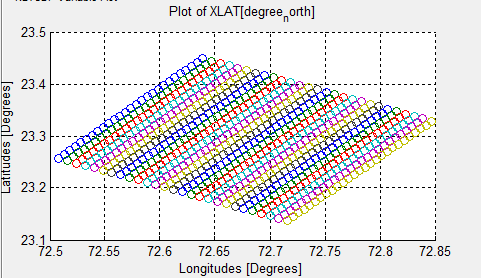
\includegraphics[scale=0.5]{LAT_LONG_GSEC}
\caption{GSEC 1MW WRF Simulation-Latitude Longitude Grid}
\label{WRFResImg1} %% to refer use, \ref{}
\end{figure}

\begin{figure}[H]
\centering
\includegraphics[scale=0.5]{U10_NETCDF_GSEC}
\caption{GSEC 1MW WRF Simulation-10m Wind Velocity (u-Component) Grid}
\label{WRFResImg2} %% to refer use, \ref{}
\end{figure}

\begin{figure}[H]
\centering
\includegraphics[scale=0.5]{V10_NETCDF_GSEC}
\caption{ GSEC 1MW WRF Simulation-10m Wind Velocity (v-Component) Grid}
\label{WRFResImg3} %% to refer use, \ref{}
\end{figure}

\begin{figure}[H]
\centering
\includegraphics[scale=0.5]{T2_NETCDF_GSEC}
\caption{ GSEC 1MW WRF Simulation-2m Temperature Grid}
\label{WRFResImg4} %% to refer use, \ref{}
\end{figure}

\begin{figure}[H]
\centering
\includegraphics[scale=0.5]{SWDOWN_NETCDF_GSEC}
\caption{ GSEC 1MW WRF Simulation- Short Wave Downward Flux Grid}
\label{WRFResImg5} %% to refer use, \ref{}
\end{figure}


\subsection{Forecasting Results}
\
\
\
\
The WRF software has been run for the entire month of June,2016 with initialization data acquired from NCEP FTP server for the region consisting of the GSEC 1MW SPVP, Gandhinagar, Gujarat at a spatial resolution of 1km and a temporal resolution of 15 minutes. The results thus obtained have been extracted from the NETCDF wrf.out files into excel files for the latitude and longitude of the GSEC SPVP using the WRF-NETCDF Visualization and Extraction App. The variables extracted are the 10m Wind Speed (U and V direction), 2m Temperature and the Short-Wave Downward Flux. Out of these the wind speed files have been processed to give  a single wind speed for the desired grid cell, and the temperature in Kelvin has been converted to $^{\circ}$C. These converted excel files have been fed as input to the solar energy estimation app and the energy forecast have been generated. The following sections illustrate graphs of the weather variables generated by WRF and the energy forecast generated from the solar energy estimation app, and their comparison with the actual weather and energy output data of the GSEC SPVP for the month of June, 2015 (due to unavailability of recent data). The graphs for the dates 5, 10, 15, 20, 25 have been shown.

\newpage


\subsubsection{5^{th} \textbf{June, 2016:}}
\
\
\
\

\begin{figure}[H]
\centering
\includegraphics[scale=0.5]{WRFw5}
\caption{Comparision Of Actual And WRF Generated Wind Speed For 5th June}
\label{WRFResImg6} %% to refer use, \ref{}
\end{figure}

\begin{figure}[H]
\centering
\includegraphics[scale=0.5]{WRFt5}
\caption{Comparision Of Actual And WRF Generated Temperature For 5th June}
\label{WRFResImg7} %% to refer use, \ref{}
\end{figure}

\begin{figure}[H]
\centering
\includegraphics[scale=0.5]{WRFi5}
\caption{Comparision Of Actual And WRF Generated Irradiance For 5th June}
\label{WRFResImg8} %% to refer use, \ref{}
\end{figure}

\begin{figure}[H]
\centering
\includegraphics[scale=0.5]{WRFe5}
\caption{Comparision Of Actual And WRF Generated Energy For 5th June}
\label{WRFResImg9} %% to refer use, \ref{}
\end{figure}


\subsubsection{10^{th} \textbf{June, 2016:}}
\
\
\
\

\begin{figure}[H]
\centering
\includegraphics[scale=0.5]{WRFw10}
\caption{ Comparision Of Actual And WRF Generated Wind Speed For 10th June }
\label{WRFResImg10} %% to refer use, \ref{}
\end{figure}

\begin{figure}[H]
\centering
\includegraphics[scale=0.5]{WRFt10}
\caption{Comparision Of Actual And WRF Generated Temperature For 10th June}
\label{WRFResImg11} %% to refer use, \ref{}
\end{figure}

\begin{figure}[H]
\centering
\includegraphics[scale=0.5]{WRFi10}
\caption{Comparision Of Actual And WRF Generated Irradiance For 10th June}
\label{WRFResImg12} %% to refer use, \ref{}
\end{figure}

\begin{figure}[H]
\centering
\includegraphics[scale=0.5]{WRFe10}
\caption{Comparision Of Actual And WRF Generated Energy For 10th June}
\label{WRFResImg13} %% to refer use, \ref{}
\end{figure}



\subsubsection{15^{th} \textbf{June, 2016:}}
\
\
\
\

\begin{figure}[H]
\centering
\includegraphics[scale=0.5]{WRFw15}
\caption{Comparision Of Actual And WRF Generated Wind Speed For 15th June }
\label{WRFResImg14} %% to refer use, \ref{}
\end{figure}

\begin{figure}[H]
\centering
\includegraphics[scale=0.5]{WRFt15}
\caption{Comparision Of Actual And WRF Generated Temperature For 15th June }
\label{WRFResImg15} %% to refer use, \ref{}
\end{figure}

\begin{figure}[H]
\centering
\includegraphics[scale=0.5]{WRFi15}
\caption{Comparision Of Actual And WRF Generated Irradiance For 15th June }

\label{WRFResImg16} %% to refer use, \ref{}
\end{figure}
\begin{figure}[H]
\centering
\includegraphics[scale=0.5]{WRFe15}
\caption{Comparision Of Actual And WRF Generated Energy For 15th June}
\label{WRFResImg17} %% to refer use, \ref{}
\end{figure}

\newpage

\subsubsection{20^{th} \textbf{June, 2016:}}
\
\
\
\

\begin{figure}[H]
\centering
\includegraphics[scale=0.5]{WRFw20}
\caption{Comparision Of Actual And WRF Generated Wind Speed For 20th June}
\label{WRFResImg18} %% to refer use, \ref{}
\end{figure}

\begin{figure}[H]
\centering
\includegraphics[scale=0.5]{WRFt20}
\caption{Comparision Of Actual And WRF Generated Temperature For 20th June}
\label{WRFResImg19} %% to refer use, \ref{}
\end{figure}

\begin{figure}[H]
\centering
\includegraphics[scale=0.5]{WRFi20}
\caption{Comparision Of Actual And WRF Generated Irradiance For 20th June}
\label{WRFResImg20} %% to refer use, \ref{}
\end{figure}

\begin{figure}[H]
\centering
\includegraphics[scale=0.5]{WRFe20}
\caption{Comparision Of Actual And WRF Generated Energy For 20th June}
\label{WRFResImg21} %% to refer use, \ref{}
\end{figure}


\subsubsection{25^{th} \textbf{June, 2016:}}
\
\
\
\

\begin{figure}[H]
\centering
\includegraphics[scale=0.5]{WRFw25}
\caption{Comparision Of Actual And WRF Generated Wind Speed For 25th June}
\label{WRFResImg22} %% to refer use, \ref{}
\end{figure}

\begin{figure}[H]
\centering
\includegraphics[scale=0.5]{WRFt25}
\caption{Comparision Of Actual And WRF Generated Temperature For 25th June}
\label{WRFResImg23} %% to refer use, \ref{}
\end{figure}

\begin{figure}[H]
\centering
\includegraphics[scale=0.5]{WRFi25}
\caption{Comparision Of Actual And WRF Generated Irradiance For 25th June}
\label{WRFResImg24} %% to refer use, \ref{}
\end{figure}

\begin{figure}[H]
\centering
\includegraphics[scale=0.5]{WRFe25}
\caption{Comparision Of Actual And WRF Generated Energy For 25th June}
\label{WRFResImg25} %% to refer use, \ref{}
\end{figure}

\subsubsection{Conclusion from Graphs}
\
\
\
\
The graphs shown in the previous sections show that the WRF is able to compute the weather variables approximately for the desired SPVP location. It is not able to model the sharp dips in the irradiances which are caused by cloud movement (prediction of cloud movements is poor in WRF). However, when the actual irradiance graphs have no significant sharp dips i.e. clouds are not present, then the WRF irradiance is slightly over estimated (due to poor modeling of aerosols). Overall, WRF shows potential for a day-ahead forecast which can be improved further by improved parameterization and appropriate physics option selection based on the region of forecast.